\documentclass[12pt,letterpaper]{article}

\usepackage[spanish,es-tabla,es-nodecimaldot]{babel}
\usepackage{amsmath}
\usepackage[utf8]{inputenc}
\usepackage[T1]{fontenc}
\usepackage{lmodern}
\usepackage{graphicx}
\usepackage{listings}
\usepackage{anysize} 
\usepackage{fancyhdr}
\usepackage{amsmath}
\usepackage{pdfpages}
\usepackage{graphics}
\usepackage{capt-of}
\usepackage{tabularx}
\usepackage[colorlinks=true,plainpages=true,citecolor=blue,linkcolor=blue]{hyperref}

\marginsize{2cm}{2cm}{2cm}{2cm}
\pagestyle{fancy}
\fancyhf{Líneas de transmisión y antenas}
\fancyhead[L]{\footnotesize UPIITA-IPN} 
\fancyhead[R]{\footnotesize 3TV1} 
\fancyfoot[R]{\footnotesize Tarea}
\fancyfoot[C]{\thepage}
\fancyfoot[L]{\footnotesize Parametros de una antena} 

\renewcommand{\footrulewidth}{0.4pt}
\renewcommand{\spanishtablename}{Tabla}
\renewcommand{\labelitemii}{$\star$}

\begin{document}
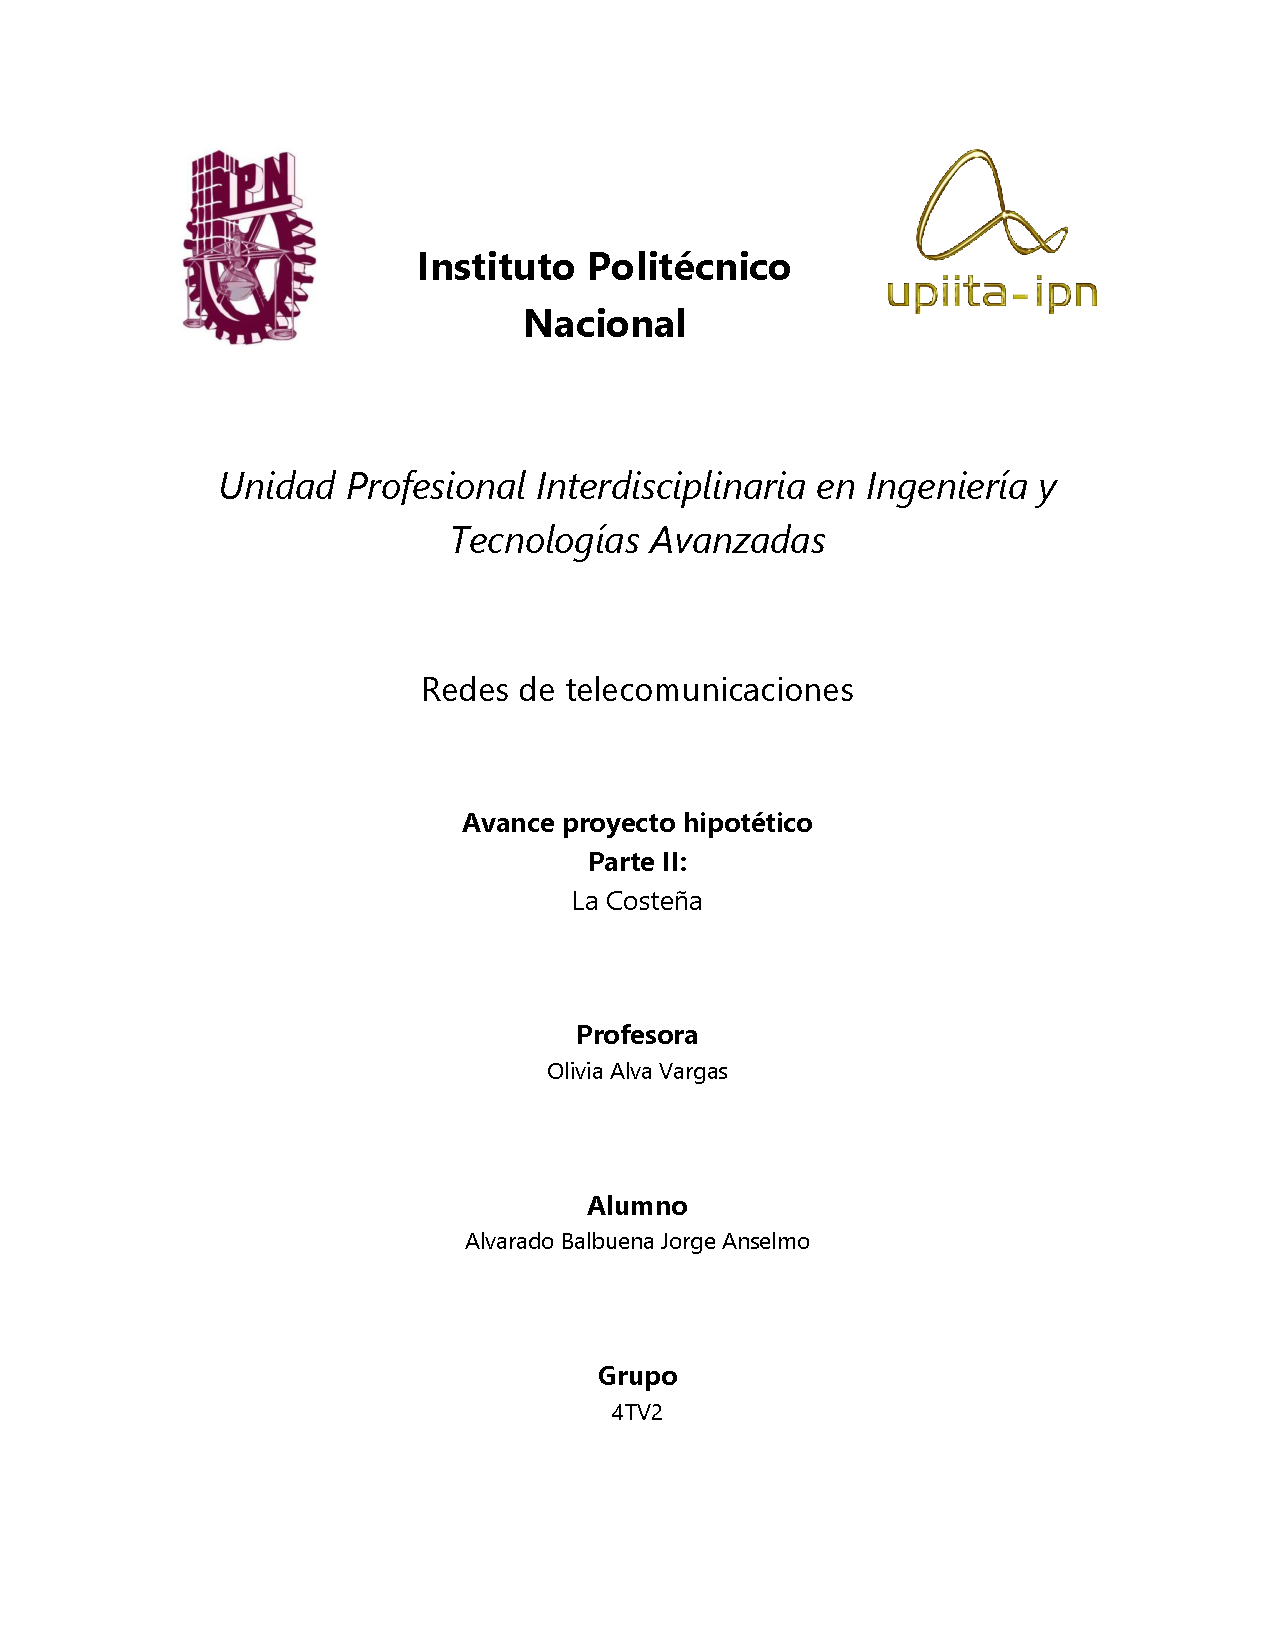
\includepdf[pages={1}]{portada2}

\newpage
\tableofcontents
\listoffigures
\listoftables


\newpage
\section{Ancho de banda}
La IEEE define el ancho de banda como \"el rango de frecuencias dentro de la cual la 
calidad de funcionamiento de la antena, con respecto a alguna característica, se ajusta 
a una norma especificada\".  El ancho de banda depende de la eficacia global de la antena 
a través de una gama de frecuencias, por lo que debe entenderse que todos estos parámetros 
caracterizan plenamente las capacidades de ancho de banda de una antena. En la práctica, 
el ancho de banda se determina normalmente midiendo una característica como la ROE o la 
potencia radiada en el rango de frecuencias de interés. Por ejemplo, el ancho de banda de 
la ROE se determina normalmente midiendo la gama de frecuencias en la que la ROE es 
inferior a 2:1. Otro valor frecuentemente utilizado para determinar el ancho de banda de 
las antenas resonantes es el valor de pérdida de retorno de -3dB \cite{anchobanda}. 
\\ \\
El ancho de banda también puede describirse en términos de porcentaje de la frecuencia 
central de la banda.
\begin{equation}
    BW=100 * \frac{F_H-F_L}{F_C}
\end{equation}
\\
Donde $F_H$ es la frecuencia más alta de la banda, $F_L$ es la frecuencia más baja de 
la banda y $F_C$ es la frecuencia central de la banda. De esta manera, el ancho de banda 
es constante en relación con la frecuencia. Si el ancho de banda se expresara en unidades 
absolutas de frecuencia, sería diferente dependiendo de la frecuencia central. Los 
diferentes tipos de antenas tienen diferentes limitaciones de ancho de banda. 

\section{Patrón de radiación}
El patrón de radiación describe la intensidad relativa del campo radiado en varias 
direcciones desde la antena, a una distancia constante. El patrón de radiación es también 
un patrón de recepción, ya que también describe las propiedades de recepción de la antena. 
El patrón de radiación es tridimensional, pero generalmente los patrones de radiación 
medidos son un corte bidimensional del patrón tridimensional, en los planos horizontal o 
vertical. Estas medidas de patrones se presentan en formato rectangular o polar. 
\\ \\
Hay dos tipos de patrón de radiación: absoluto y relativo. Los diagramas absolutos de 
radiación se presentan en unidades absolutas de intensidad de campo o potencia. Los 
diagramas de radiación relativos se refieren en unidades relativas de intensidad de 
campo o potencia. La mayoría de las mediciones del diagrama de radiación son relativas a 
la antena isotrópica, y luego se utiliza el método de transferencia de ganancia para 
establecer la ganancia absoluta de la antena.
\\ \\ 
El patrón de radiación en la región cercana a la antena no es el mismo que el patrón 
a grandes distancias. El término campo cercano se refiere al patrón de campo que existe 
cerca de la antena, mientras que el término campo lejano se refiere al patrón de campo 
a grandes distancias. El campo lejano también se llama campo de radiación, y es lo que 
más comúnmente interesa. Normalmente, lo que interesa es la potencia radiada, por lo que 
los diagramas de antena se miden normalmente en la región de campo lejano. Para la 
medición de patrones es importante elegir una distancia lo suficientemente grande para 
estar en el campo lejano, bien fuera del campo cercano. La distancia mínima admisible 
depende de las dimensiones de la antena en relación con la longitud de onda. La fórmula 
aceptada para esta distancia es:
\begin{equation}
    r_{min}=\frac{2d^2}{\lambda}
\end{equation}
donde $r_{min}$ es la distancia mínima desde la antena, $d$ es la mayor dimensión de la 
antena, y $\lambda$ es la longitud de onda \cite{radiacion}. 

\section{Polzarización}
La polarización se define como la orientación del campo eléctrico de una onda 
electromagnética. La polarización se describe en general mediante una elipse. Dos casos 
especiales de polarización elíptica son la polarización lineal y la polarización circular. 
La polarización inicial de una onda de radio está determinada por la antena.
\\ \\
Con la polarización lineal, el vector del campo eléctrico permanece en el mismo plano 
todo el tiempo. La radiación de polarización vertical se ve algo menos afectada por las 
reflexiones sobre el trayecto de transmisión. Las antenas omnidireccionales siempre 
tienen polarización vertical. 
\\ \\
Con la polarización horizontal, tales reflexiones causan variaciones en la intensidad de 
la señal recibida. Las antenas horizontales tienen menos probabilidades de detectar 
interferencias causadas por el hombre, que normalmente están polarizadas verticalmente. 
\\ \\
En la polarización circular, el vector del campo eléctrico parece estar girando con un 
movimiento circular sobre la dirección de propagación, haciendo un giro completo para 
cada ciclo. Esta rotación puede ser a la derecha o a la izquierda. La elección de la 
polarización es una de las opciones de diseño disponibles para el diseñador del sistema 
de radiofrecuencia. 
\\ \\ 
Para transferir la máxima potencia entre una antena transmisora y una receptora, 
ambas antenas deben tener la misma orientación espacial, el mismo sentido de polarización 
y la misma relación axial. Cuando las antenas no están alineadas o no tienen la misma 
polarización, habrá una reducción en la transferencia de potencia entre las dos antenas. 
Esta reducción en la transferencia de potencia reducirá la eficiencia y el rendimiento 
general del sistema. Si las polarizaciones conciden, no se produce ninguna atenuación debido al 
desajuste de acoplamiento entre el campo y la antena, mientras que si no lo son, 
entonces la comunicación ni siquiera puede tener lugar \cite{polarizacion}.

\newpage
\section{Ganancia}
La ganancia de una antena es la relación entre la intensidad de radiación en una dirección 
dada y la intensidad de radiación que se obtendría si la potencia aceptada por la antena 
fuera irradiada isótropa.
\\ \\
Simplemente, la ganancia de una antena tiene en cuenta la directividad de la antena junto 
con su rendimiento efectivo. Si la potencia aceptada por la antena fue irradiada isótropa 
(es decir, en todas las direcciones), entonces la intensidad de radiación que obtenemos 
puede ser tomada como referencial.
\begin{itemize}
    \item El término ganancia de antena describe cuánta potencia se transmite en la 
    dirección de la radiación máxima a la de una fuente isotrópica.
    \item La ganancia se mide normalmente en dB.
    \item La ganancia de la antena tiene en cuenta las pérdidas que se producen y, 
    por lo tanto, se centra en la eficiencia \cite{polarizacion}.
\end{itemize}

\section{Impedancia de entrada}
La impedancia relaciona el voltaje y la corriente en la entrada de la antena. La 
parte real de la impedancia de la antena representa la potencia que se irradia o se 
absorbe dentro de la antena. La parte imaginaria de la impedancia representa la potencia 
que se almacena en el campo cercano de la antena. Esto es energía no irradiada. Se dice 
que una antena con una impedancia de entrada real (parte imaginaria cero) es resonante. 
Se debe tener en cuenta que la impedancia de una antena variará con la frecuencia. Para 
una transferencia eficiente de energía, la impedancia de la antena y del cable de 
transmisión que los conecta debe ser la misma \cite{polarizacion}. 

\newpage
\section{Ancho de haz a media potencia}
La separación angular, en la que la magnitud del patrón de radiación disminuye en un 
50\% (-3dB) desde el pico del haz principal, es el ancho de haz de media potencia. El 
ancho del haz es el área donde se irradia la mayor parte de la potencia, que es la 
potencia máxima. La anchura del haz de media potencia es el ángulo en el que la potencia 
relativa es superior al 50\% de la potencia máxima en el campo radiado efectivo de la antena.
\\ \\
Cuando se traza una línea entre el origen del diagrama de radiación y los puntos de 
media potencia en el lóbulo mayor, a ambos lados, el ángulo entre esos dos vectores se 
denomina HPBW, la mitad del ancho del haz de potencia. Esto se puede entender bien con 
la ayuda del siguiente diagrama \cite{haz}.

\newpage
\begin{thebibliography}{20}
    \bibitem{anchobanda}
    IEEE Standard Definitions of Terms for Antennas, in IEEE Std 145-1993 , vol., no., pp.1-32, 18 July 1993

    \bibitem{radiacion}
    Constantine A. Balanis: Antenna Theory, Analysis and Design, John Wiley and Sons, Inc., 2nd ed. 1982.
    
    \bibitem{polarizacion}
    Constantine A. Balanis: Modern Antenna Handbook, Wiley, 2007.

    \bibitem{haz}
    W. L. Stutzman and G. A. Theile, Antenna theory and design. John Wiley and Sons, Inc., 1998.
\end{thebibliography}

\end{document}